\documentclass[letterpaper,10pt,conference]{ieeeconf}
\IEEEoverridecommandlockouts

\usepackage{graphicx,amsmath,amssymb,booktabs,multirow,cite,url,array,xcolor,colortbl,tabularx}
\usepackage[protrusion=false]{microtype}
\usepackage{caption}
\usepackage{hyperref}

\newcommand{\ours}{TactiOS}
\newcommand{\sensor}{GelSlim~5.0}
\newcommand{\todo}[1]{\textcolor{red}{[#1]}}
\newcommand{\tableformat}{\small\setlength{\tabcolsep}{3.0pt}\renewcommand{\arraystretch}{1.02}}
\newcommand{\metrichead}[2]{\shortstack[c]{\strut#1\\\strut#2\,$\downarrow$}}
\newcommand{\Kreal}{K}

\title{\LARGE\bf How Much Real Data Does a Tactile Renderer Need?\\
A Leakage-Controlled Real-to-Sim-to-Real Study of Tactile Depth and Pose Estimation}

\author{I-Hsuan Huang$^{*}$, Xiaohao Xu$^{*}$, Xiangdong Wang, Xiaonan Huang, and Nima Fazeli%
\thanks{$^{*}$Equal contribution. All authors are with the University of Michigan, Ann Arbor, MI, USA.
Correspondence: \texttt{\{ihsuan, xiaohaox\}@umich.edu}.}%
}

\begin{document}
\maketitle
\thispagestyle{empty}
\pagestyle{empty}

\begin{abstract}
Vision-based tactile sensors image a deforming elastomer under internal illumination, so the mapping from contact geometry to appearance is sensor specific and dense real labels are expensive. Real-to-sim-to-real pipelines calibrate a tactile renderer on a little real data and train on its synthetic labels. We ask what such pipelines rarely control for: \emph{how much real data does the renderer itself consume, and does the downstream gain survive once that data is accounted for?} On one \sensor{} sensor and one downstream model (frozen sensor-invariant encoder with depth, normal and planar-pose heads) we compare a \emph{physically calibrated} Blender renderer, fitted by Bayesian optimization to a single no-contact image, with a \emph{learned} depth-to-image renderer trained on $\Kreal$ real pairs per object, under a leakage-controlled protocol in which the renderer never sees the frames used to test the downstream model. Simulation is decisive for \emph{pose transfer to new objects}: with no real data of three objects, rotation error drops from $48^\circ$ to $5.6^\circ$ once simulated contacts of their meshes are added, using the physical renderer and no real contact of the object; a control that removes the meshes from simulation shows the gain is geometric coverage, not appearance. For \emph{dense contact depth} the benefit is gated by appearance fidelity: the learned renderer needs $\Kreal\!\ge\!100$ pairs per object before synthetic data lowers real depth error ($-18\%$ MSE, $-15\%$ contact MAE), the physical renderer never does, and the common leaky practice of training the renderer on all real data overstates the gain by up to $2\times$. A contact-region L1 between rendered and real images predicts the downstream ranking, and physics pretraining, illumination normalization and difference-image rendering all fail to close the few-shot gap, locating the bottleneck in contact shading rather than illumination drift.
\end{abstract}

\section{Introduction}

Vision-based tactile sensors such as GelSight, GelSlim and DIGIT~\cite{yuan2017gelsight,donlon2018gelslim,lambeta2020digit} measure contact by imaging a soft elastomer under internal colored illumination. The image is not a picture of the object: it is the result of gel deformation, LED placement and color, elastomer reflectance, camera response and manufacturing variation. Two sensors of the same design, or the same sensor across sessions, produce different images for the same contact. Dense perception from these images---contact depth, surface normals, object pose---therefore needs sensor-specific supervision, and dense real labels are expensive to obtain.

Real-to-sim-to-real pipelines address this by \emph{calibrating a tactile renderer} on a small amount of real data and then training on synthetic images whose depth, normal and pose labels come for free~\cite{si2022taxim,wang2022tacto,chen2023tacchi,zhong2025tactgen}. Two renderer families are in use. \emph{Physically calibrated} renderers keep a light-transport model of the sensor and fit its parameters---LED color and strength, gel material, camera response---to real images~\cite{agarwal2021simulation,si2022taxim}. \emph{Learned} renderers replace the light-transport model by an image-to-image network trained on real (depth, image) pairs~\cite{zhong2025tactgen}. The two families sit at opposite ends of a data-efficiency axis: a physical renderer can be calibrated from a single no-contact frame, whereas a learned renderer needs labeled contact pairs, i.e. exactly the data the pipeline is meant to save.

This paper asks how much real data each renderer needs before its synthetic data improves a downstream tactile model, and whether the reported gains survive a control that is usually missing: the renderer must not see the real frames on which the downstream model is tested. In many learned-renderer pipelines the renderer is trained on all available real pairs and the downstream model is validated on frames from the same sessions; the renderer has then memorized the appearance of the test contacts, and the synthetic data carries that information into training. We show this \emph{leakage} inflates the measured benefit by up to a factor of two.

We study the question on \sensor{}, a GelSlim-type fingertip sensor, with a single downstream architecture (a frozen sensor-invariant tactile encoder~\cite{gupta2025sitr} with dense depth/normal and planar-pose heads) and two renderers built on the same object meshes and contact sampler: a Blender renderer calibrated by Bayesian optimization to one no-contact image, and a pix2pix depth-to-image renderer~\cite{isola2017pix2pix,church2022tactile} trained on $\Kreal$ real pairs per object. We evaluate under two protocols. \emph{Leave-object-out} holds out three objects with no real data at all and asks whether simulated contacts of their meshes transfer. \emph{$\Kreal$-shot} gives every object $\Kreal\in\{0,10,25,100\}$ real frames, and---critically---trains the learned renderer on the same $\Kreal$ frames as the downstream model.

Our findings are:
\begin{enumerate}
    \item \textbf{Simulation is decisive for pose transfer to new objects.} With no real data of an object, a tactile pose model fails ($48^\circ$ mean rotation error). Adding simulated contacts of the object's mesh reduces this to $5.6^\circ$ with the physically calibrated renderer and $6.3^\circ$ with the strict learned renderer. A control that keeps the renderer but removes the held-out geometry from simulation stays at $55^\circ$: the benefit is geometric coverage, and the renderer's appearance fidelity is secondary.
    \item \textbf{For dense depth, the benefit is gated by appearance fidelity and by $\Kreal$.} The physically calibrated renderer does not lower real depth error at any $\Kreal$. The learned renderer lowers it only from $\Kreal=100$ pairs per object ($-18\%$ MSE, $-15\%$ contact-region MAE, $+0.04$ contact IoU); at $\Kreal\le 25$ it is indistinguishable from training on the real frames alone. Few-shot depth error is dominated by overfitting to the few real frames, not by the amount of synthetic data.
    \item \textbf{Leakage matters.} A learned renderer trained on all real pairs appears to cut depth error by $24$--$31\%$ at every $\Kreal$ and on unseen objects; under the strict protocol the gain is $0$--$18\%$. We recommend reporting learned-renderer results with the renderer's training frames disjoint from the downstream test frames.
    \item \textbf{A cheap fidelity proxy predicts downstream ranking.} The contact-region L1 between rendered and real images on held-out pairs orders eight renderer variants the same way as their downstream depth error, so renderer design can be iterated in minutes rather than hours.
    \item \textbf{Negative results on the appearance side.} Pretraining the learned renderer on the physical renderer's images, normalizing per-session illumination drift (which we measure to be larger than the renderer error itself), and predicting difference images all fail to improve small-$\Kreal$ fidelity in the contact region, locating the bottleneck in contact shading rather than in the illumination field.
\end{enumerate}

\section{Related Work}

\noindent\textbf{Vision-based tactile sensing.}
GelSight-type sensors convert elastomer deformation into images under structured illumination~\cite{johnson2009retrographic,yuan2017gelsight}; GelSlim~\cite{donlon2018gelslim,sipos2024gelslim4} and DIGIT~\cite{lambeta2020digit} adapt the principle to fingertips. Because the measurement depends jointly on gel mechanics, LED layout and camera response, models transfer poorly between sensors; sensor-invariant representations~\cite{gupta2025sitr,zhao2024transferable,higuera2024sparsh,higuera2025sparshx} and deformation-space translation~\cite{zai2025across,yang2025flow} attack this on the representation side. We use a frozen sensor-invariant encoder~\cite{gupta2025sitr} as backbone so that our comparison isolates the data.

\noindent\textbf{Tactile simulation.}
Physically based tactile renderers synthesize GelSight images from mesh contacts~\cite{agarwal2021simulation,wang2022tacto,luu2023simulation}, with example-based~\cite{si2022taxim}, particle-based~\cite{chen2023tacchi}, differentiable~\cite{xu2022efficient} and GPU-scale~\cite{nguyen2024tacex,akinola2025tacsl} variants. Learned renderers instead map simulated depth or contact state to sensor images with an image-to-image network~\cite{isola2017pix2pix,church2022tactile,zhong2025tactgen}. Our two renderers follow the two lines and share meshes, contact sampler and labels, so they differ only in the appearance model.

\noindent\textbf{Sim-to-real transfer and its evaluation.}
Domain randomization~\cite{tobin2017domain,peng2018sim} and structured randomization around a calibrated center~\cite{chen2024general} trade fidelity for robustness; sensor-background conditioning~\cite{zhong2025tactgen} and low-fidelity pretraining~\cite{gano2025lowfidelity} report gains from synthetic tactile data. These works measure the benefit of simulation but rarely report how much real data the simulator consumed, or whether the simulator saw the test distribution. Cross-sensor transfer is usually attacked on the representation side~\cite{gupta2025sitr,zhao2024transferable}; we instead ask how much of a new sensor's or session's real data a renderer needs. Our contribution is the evaluation protocol---renderer and downstream model trained on the same disjoint real subset, tested on held-out objects, a second session and a second sensor---and the resulting data-efficiency curves for depth, normals and pose with both renderer families.

\section{Real-to-Sim-to-Real Pipeline}
\label{sec:method}

\begin{figure*}[t]
    \centering
    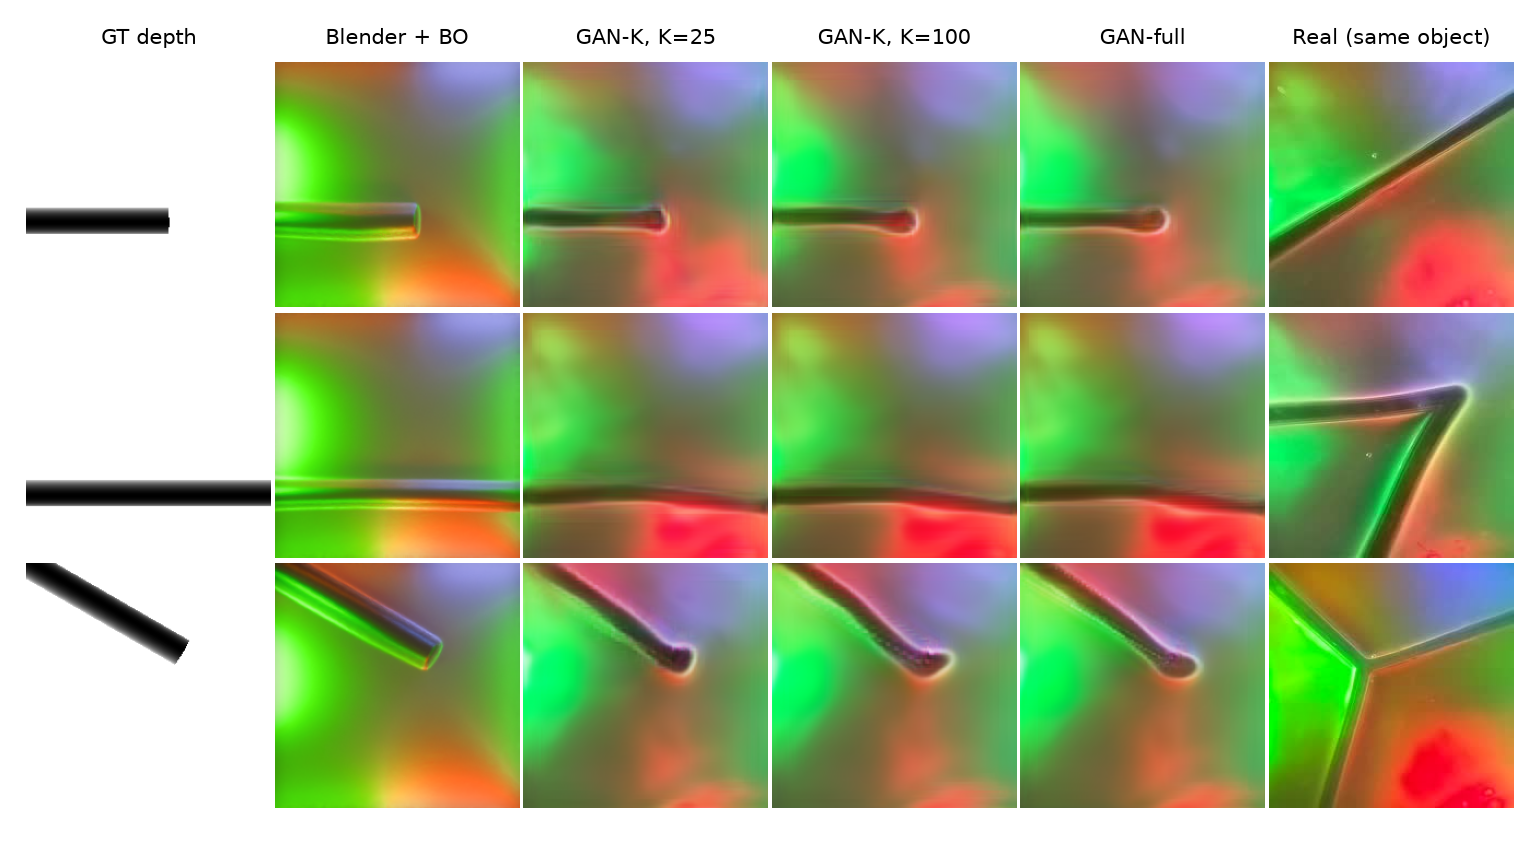
\includegraphics[width=0.96\textwidth]{figures/fig_renders.png}
    \caption{\textbf{Two renderers, one contact.} Each row is one simulated contact (GT depth, left) rendered by the physically calibrated Blender renderer, by the learned renderer trained on $\Kreal=25$ or $\Kreal=100$ real pairs per object, and by the learned renderer trained on all real pairs (GAN-full). The right column shows a real frame of the same object. The physical renderer reproduces the illumination field but not the dark, low-contrast contact shading of the real gel; the learned renderers reproduce the shading and inherit the mean illumination field of their training frames.}
    \label{fig:renders}
\end{figure*}

\subsection{Problem Statement}
Let $M$ be an object mesh and $q$ a contact state (planar pose of the object relative to the sensor and indentation depth). A tactile renderer $\mathcal{R}_\theta$ maps $(M,q)$ to an image and dense labels,
\begin{equation}
    (\hat I, D, N) = \mathcal{R}_\theta(M,q),
\end{equation}
where $D$ is the contact depth map, $N$ the surface normal map and $\theta$ the appearance parameters. The geometry part $\mathcal{G}:(M,q)\mapsto(D,N)$ is shared by every renderer we study; renderers differ only in the appearance operator $\mathcal{P}_\theta:(D,N)\mapsto\hat I$ and in the real data $\mathcal{D}^{r}_{\mathrm{cal}}$ used to fit $\theta$. A downstream model $f_\phi$ predicts $(\hat D,\hat N,\hat p)$ from a real image, with $p$ the planar pose. We measure the utility of a renderer by the real test error of $f_\phi$ after training on synthetic data $\mathcal{D}_{\mathrm{sim}}^{\theta}$ together with a real subset $\mathcal{D}^{r}_{\mathrm{task}}$, and we control the total real budget $\mathcal{D}^{r}_{\mathrm{cal}}\cup\mathcal{D}^{r}_{\mathrm{task}}$.

\subsection{Sensor and Data}
\noindent\textbf{Sensor.} We use \sensor{}, a GelSlim-type fingertip sensor with a $17.5\,$mm square gel view imaged by an internal camera under six colored LED emitters. Images are center-cropped to $0.816$ of the view and resized to $224\times224$.

\noindent\textbf{Real data.} A KUKA LBR Med arm presses the sensor onto 12 ridge-pattern objects (line, cross and rod patterns of known geometry), recording the tactile image and end-effector pose at every contact. A reference-object calibration relates object pose to the sensor frame; depth and normal references are computed from the mesh at the recorded pose, so they are geometric targets rather than membrane measurements. After filtering frames whose image-derived contact region disagrees with the reference (IoU $<0.3$), $4{,}669$ frames remain ($222$--$568$ per object). Each object was captured in one session, so \emph{object identity and capture session coincide}; we return to this in Sec.~\ref{sec:negative}. Every tenth frame is held out as the real validation split ($472$ frames).

\noindent\textbf{Contact sampler.} For each object we sample contact cells over the mesh at 12 base rotations ($30^\circ$ apart), an indentation depth of $0.8$--$1.2\,$mm and a small in-plane jitter, and export the depth map $D$ from the object z-buffer and $N$ by finite differences. Simulated poses are restricted to each object's real rotation and translation ranges (margin $1.5\times$). The same $5{,}345$ simulated contacts feed every renderer.

\subsection{Physically Calibrated Renderer}
\label{sec:blender}
The physical renderer is implemented in Blender/Cycles. Gel deformation is geometric: a gel surface mesh is shrink-wrapped onto the object along the sensor normal and smoothed with 35 corrective-smoothing iterations to mimic elastomer stiffness. The gel material is a glossy/transparent mix (roughness $0.45$, glossy fraction $0.17$) with a contact-darkening term driven by gel height. Illumination comes from six area emitters with individual strength and RGB color. A post-processing stage adds saturation, brightness, contrast, haze and a low-frequency gel-warp field.

\noindent\textbf{Calibration from one frame.} Following the base-field alignment of inverse tactile rendering, we fit $\theta_{\mathrm{illum}}\cup\theta_{\mathrm{post}}$ (three emitters $\times$ (strength, R, G, B) plus four post-processing scalars; 16 parameters) by minimizing
\begin{equation}
    \mathcal{L}_{\mathrm{base}} = 0.6\,\|B^{r}-\hat B_\theta\|_2^2 + 0.4\,D_{\mathrm{Bhat}}\!\left(H(B^{r}),H(\hat B_\theta)\right)
\end{equation}
between the real no-contact image $B^{r}$ and the rendered one, with $H$ the per-channel histogram and $D_{\mathrm{Bhat}}$ the Bhattacharyya distance, using tree-based Bayesian optimization (500 evaluations, warm-started from manual tuning). The remaining gel and contact parameters were tuned by hand on a few contact frames. The real budget of this renderer is therefore \emph{one no-contact frame}, and it never sees a labeled contact.

\subsection{Learned Renderer}
\label{sec:gan}
The learned renderer replaces $\mathcal{P}_\theta$ by a conditional GAN~\cite{isola2017pix2pix,church2022tactile}. The generator is a five-level U-Net taking the depth map and two CoordConv coordinate channels (the illumination field is a function of position) and producing an RGB image; the discriminator is a $70\times70$ PatchGAN with spectral normalization on the (depth, image) pair. The loss is adversarial + $100\,(\mathrm{L1} + \mathrm{gradient\;L1} + \mathrm{low\text{-}frequency\;L1})$. At data-generation time the simulated depth is jittered by $\pm15\%$ before rendering.

\noindent\textbf{Real budget.} We train one generator per budget: GAN-$\Kreal$ uses $\Kreal$ real (depth, image) pairs per object, drawn as an evenly spaced subset of each object's training frames; GAN-LOO uses all training frames of the 9 non-held-out objects; GAN-full uses all $4{,}197$ training pairs. Small budgets are trained for at least $30$k generator updates. The GAN-$\Kreal$ subset is by construction \emph{the same} $\Kreal$ frames the downstream model later receives (Sec.~\ref{sec:protocol}).

\subsection{Downstream Tactile Model}
The downstream model is deliberately simple and identical for every renderer: a frozen sensor-invariant tactile encoder (SITR-B/18~\cite{gupta2025sitr}, ViT-B/16, 18 calibration images) provides patch tokens at four depths; a DPT decoder~\cite{ranftl2021dpt} predicts depth and normals at $224\times224$; a pose head pools the class token with the mean patch token and regresses $(\cos\theta,\sin\theta,t_x,t_y)$. Only the decoder, pose head and a learned object embedding are trained ($12$M parameters). Losses are MSE on depth and normals, $1-\cos(\theta-\hat\theta)$ on rotation and L1 on translation, balanced by grouped uncertainty weighting~\cite{kendall2018multi}. Training co-mixes simulated and real frames in one dataset; simulated frames receive photometric augmentation (gain, bias, gradient, noise) and $\pm15^\circ$ gel-spin rotation with matched label rotation, real frames receive none. AdamW, learning rate $2\times10^{-4}$, batch 32, cosine schedule with 1k warm-up steps. \todo{Pilot tables use 50 epochs; final tables will use 150 epochs (runs in progress). A 150-epoch check on four key configurations changed no conclusion.}

\subsection{Leakage-Controlled Protocol}
\label{sec:protocol}
Two protocols, one rule: \emph{no frame used to evaluate $f_\phi$ is ever seen by the renderer.}

\noindent\textbf{Leave-object-out (LOO).} Three objects (a two-line, a rod and a cross pattern; $1{,}244$ frames) are removed from all real training. They are never used to calibrate a renderer, never appear as real frames in downstream training, and are evaluated in full. Checkpoints are selected on the validation split of the nine remaining objects. Simulated contacts of the three meshes are available to every renderer, mimicking the deployment case ``new object with a CAD model but no real touches''. A \emph{geometry control} additionally removes the three meshes from simulation.

\noindent\textbf{$\Kreal$-shot.} Every object contributes $\Kreal\in\{0,10,25,100\}$ evenly spaced real training frames. The learned renderer is trained on exactly those frames; the downstream model co-trains on those frames plus simulated data (or on those frames alone, with the same number of updates). Evaluation is on the standard real validation split.

\noindent\textbf{Leaky reference.} To quantify the bias of the common practice, we also report GAN-full (renderer trained on all real pairs) in both protocols. In LOO its training set contains the held-out objects; in $\Kreal$-shot it contains frames adjacent to the validation frames. We mark these rows as leaky and never bold them.

\noindent\textbf{Metrics.} Depth MSE over all pixels ($\mathrm{mm}^2$), the metric used by prior work on this sensor; and, because $\approx90\%$ of pixels are non-contact background, the mean absolute error inside the reference contact region (contact MAE, mm), contact IoU (predicted depth $>0.05\,$mm vs.\ reference $>0$), and the per-frame peak-depth error. For pose: mean angular error and normalized translation L1.

\section{Experiments}
\label{sec:experiments}

We answer four questions. \textbf{Q1} Does simulated data transfer to objects with no real data, and which renderer is needed? \textbf{Q2} How does the benefit scale with the real budget $\Kreal$ for each renderer family? \textbf{Q3} How much does renderer leakage inflate the measured benefit? \textbf{Q4} Can renderer fidelity be measured without training the downstream model, and which appearance factors limit it?

All numbers are real-frame errors of the downstream model; depth MSE in $\mathrm{mm}^2$, contact MAE in mm, rotation in degrees. Depth metrics use the checkpoint with the lowest validation depth MSE and pose metrics the checkpoint with the lowest validation angular error, both selected on the seen-object validation split only.

\subsection{Q1: Transfer to Unseen Objects}
\label{sec:loo}

\begin{table}[t]
\centering
\tableformat
\caption{\textbf{Leave-object-out.} Errors on $1{,}244$ real frames of three objects with no real training data. Rows add simulated contacts of all 12 meshes to the real frames of the nine other objects, unless noted. Leaky: renderer trained on real frames of the held-out objects. Bold: best leakage-free.}
\label{tab:loo}
\begin{tabularx}{\columnwidth}{Xrrrrr}
\toprule
Training data & \metrichead{Depth}{MSE} & \metrichead{Contact}{MAE} & \shortstack[c]{\strut Contact\\\strut IoU\,$\uparrow$} & \metrichead{Rot.}{(deg)} & \metrichead{Trans.}{$L_1$} \\
\midrule
Real only (9 objects) & 0.0659 & 0.347 & 0.587 & 48.3 & 0.088 \\
+ Blender & 0.0675 & 0.352 & 0.587 & 7.8 & \textbf{0.035} \\
+ Blender, bg-norm. & 0.0662 & 0.348 & 0.591 & \textbf{5.6} & 0.036 \\
+ GAN-LOO & \textbf{0.0612} & \textbf{0.333} & \textbf{0.617} & 7.6 & 0.039 \\
\quad w/o held-out meshes & 0.0622 & 0.337 & 0.609 & 55.3 & 0.067 \\
+ diff-GAN-LOO & 0.0627 & 0.346 & 0.607 & 6.3 & 0.040 \\
\midrule
\textit{+ GAN-full (leaky)} & \textit{0.0455} & \textit{0.281} & \textit{0.677} & \textit{6.7} & \textit{0.037} \\
\midrule
\multicolumn{6}{@{}l}{\textit{Reference: same models on the nine seen objects}} \\
Real only & 0.0115 & 0.109 & 0.874 & 3.8 & 0.021 \\
+ GAN-LOO & 0.0094 & 0.106 & 0.884 & 5.8 & 0.029 \\
\bottomrule
\end{tabularx}
\end{table}

\begin{figure}[t]
    \centering
    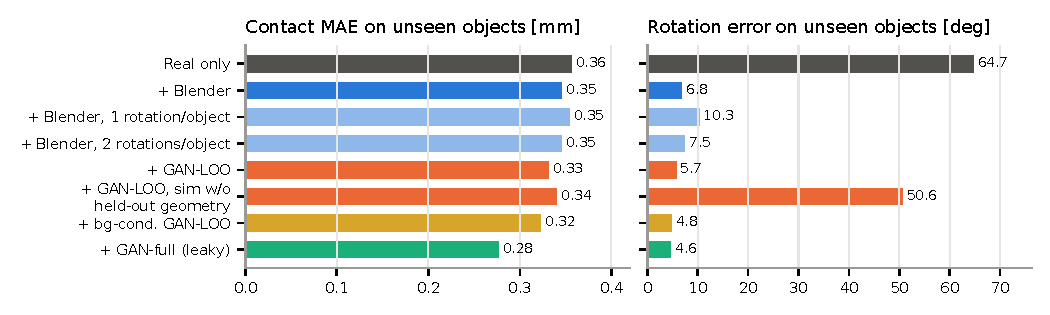
\includegraphics[width=\columnwidth]{figures/fig_loo.pdf}
    \caption{\textbf{Unseen objects (Table~\ref{tab:loo}).} Simulated contacts of a new mesh make its pose estimable with either renderer; removing the mesh from simulation (geometry control) removes the gain. Contact depth error barely moves without leakage.}
    \label{fig:loo}
\end{figure}

Table~\ref{tab:loo} and Fig.~\ref{fig:loo} give the leave-object-out results. Without any data of the three objects, the pose head fails: $48.3^\circ$ mean rotation error, which is chance level for the two-fold symmetric patterns. Adding simulated contacts of the three meshes reduces this to $7.8^\circ$ with the physically calibrated renderer---calibrated from a single no-contact frame and never shown a real contact of any object---and to $5.6^\circ$ when per-session illumination is normalized (Sec.~\ref{sec:negative}). The learned renderer reaches $7.6^\circ$ (strict) and $6.7^\circ$ (leaky); the leaky variant buys little for pose. The geometry control isolates the cause: the same GAN-LOO renderer with the three meshes removed from simulation gives $55.3^\circ$, i.e.\ no transfer. Pose transfer is driven by geometric coverage of the new object in simulation, and any renderer that preserves the contact silhouette suffices.

Dense depth behaves differently. Contact MAE on the unseen objects is $0.35\,$mm for real-only training---three times the $0.11\,$mm on seen objects---and no leakage-free renderer reduces it by more than $4\%$ (GAN-LOO: $0.333$, IoU $0.59\!\to\!0.62$). The geometry control gives almost the same depth ($0.337$), so the small gain is a regularization effect of additional synthetic frames rather than object coverage. Only the leaky renderer, which has seen real contacts of these objects, reduces contact MAE substantially ($0.281$, $-19\%$). Cross-object depth generalization is thus limited by contact appearance, and the leaky number is not achievable without real touches of the object. Peak-depth error is small for every row ($0.05$--$0.08\,$mm at $\approx1\,$mm indentation): the models estimate \emph{how deep} correctly and err in \emph{where} the contact region lies (IoU $\approx0.6$).

\subsection{Q2: Real-Data Budget}
\label{sec:kshot}

\begin{table}[t]
\centering
\tableformat
\caption{\textbf{$\Kreal$-shot with a shared real budget.} Every object contributes $\Kreal$ real frames; GAN-$\Kreal$ is trained on the same frames. Real validation split ($472$ frames). Leaky rows use the renderer trained on all real pairs.}
\label{tab:kshot}
\begin{tabularx}{\columnwidth}{lXrrrr}
\toprule
$\Kreal$ & Training data & \metrichead{Depth}{MSE} & \metrichead{Contact}{MAE} & \shortstack[c]{\strut IoU\\\strut $\uparrow$} & \metrichead{Rot.}{(deg)} \\
\midrule
0 & Blender only & 0.0786 & 0.406 & 0.574 & 9.0 \\
  & \textit{GAN-full only (leaky)} & \textit{0.0464} & \textit{0.275} & \textit{0.705} & \textit{8.0} \\
\midrule
10 & Real only & 0.0639 & \textbf{0.329} & \textbf{0.627} & 10.1 \\
   & + Blender & 0.0633 & 0.366 & 0.600 & \textbf{6.3} \\
   & + GAN-10 & \textbf{0.0620} & 0.348 & 0.596 & 6.7 \\
   & \textit{+ GAN-full (leaky)} & \textit{0.0484} & \textit{0.281} & \textit{0.693} & \textit{6.1} \\
\midrule
25 & Real only & 0.0558 & \textbf{0.303} & \textbf{0.666} & \textbf{5.5} \\
   & + Blender & 0.0569 & 0.347 & 0.659 & 5.6 \\
   & + GAN-25 & \textbf{0.0539} & 0.318 & 0.619 & 5.9 \\
   & \textit{+ GAN-full (leaky)} & \textit{0.0423} & \textit{0.254} & \textit{0.725} & \textit{5.9} \\
\midrule
100 & Real only & 0.0367 & 0.238 & 0.746 & \textbf{3.9} \\
    & + Blender & 0.0341 & 0.220 & 0.760 & 5.3 \\
    & + GAN-100 & \textbf{0.0299} & \textbf{0.202} & \textbf{0.780} & 5.5 \\
    & \textit{+ GAN-full (leaky)} & \textit{0.0273} & \textit{0.191} & \textit{0.791} & \textit{5.4} \\
\bottomrule
\end{tabularx}
\end{table}

\begin{figure*}[t]
    \centering
    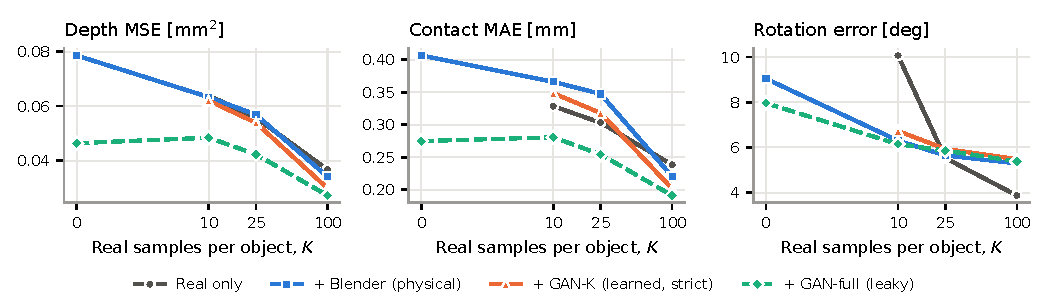
\includegraphics[width=0.95\textwidth]{figures/fig_kshot.pdf}
    \caption{\textbf{Real-data budget (Table~\ref{tab:kshot}).} Real validation error versus real frames per object. The strict learned renderer (GAN-$\Kreal$, trained on the same $\Kreal$ frames) separates from real-only training only at $\Kreal=100$; the physical renderer never improves depth. The leaky renderer (dashed) appears to help at every $\Kreal$. Rotation benefits from simulation only at $\Kreal\le10$.}
    \label{fig:kshot}
\end{figure*}

Table~\ref{tab:kshot} and Fig.~\ref{fig:kshot} vary the real budget. Three regimes appear.

\noindent\textbf{Zero-shot ($\Kreal=0$).} Simulation alone transfers poorly for depth: contact MAE $0.41\,$mm with the physical renderer, versus $0.11\,$mm reachable with the full real set. The leaky learned renderer halves this ($0.275$), but it has seen $4{,}197$ real pairs, so it is not a zero-shot result.

\noindent\textbf{Few-shot ($\Kreal\le25$).} Neither leakage-free renderer improves depth. With $\Kreal=25$, GAN-25 lowers full-image MSE by $3\%$ but \emph{raises} contact MAE ($0.303\!\to\!0.318$) and lowers IoU ($0.67\!\to\!0.62$); the physical renderer does the same. The training curves explain why: with $\Kreal\le25$ the real training loss reaches $10^{-4}$ within ten epochs while validation error is flat from epoch five, i.e.\ the model memorizes the few real frames, and synthetic frames whose contact appearance differs from the real one do not regularize that memorization. Simulation does help pose at $\Kreal=10$ ($10.1^\circ\!\to\!6.3$--$6.7^\circ$), consistent with Sec.~\ref{sec:loo}: pose needs coverage of the pose space more than appearance.

\noindent\textbf{Moderate budget ($\Kreal=100$).} The learned renderer now helps: GAN-100 reduces depth MSE from $0.0367$ to $0.0299$ ($-18\%$), contact MAE from $0.238$ to $0.202\,$mm ($-15\%$) and raises IoU from $0.75$ to $0.78$; a 150-epoch rerun confirms the gap ($0.0369$ vs.\ $0.0311$). The physical renderer gives a smaller gain ($-7\%$ MSE). The learned renderer thus needs on the order of $100$ labeled contacts per object before its synthetic data is worth more than the frames it was trained on. At every $\Kreal\ge25$, adding simulation \emph{worsens} rotation by $1$--$1.5^\circ$; the pose head prefers the real distribution once it is adequately covered, mirroring the intermediate optimal real:sim ratio reported for fusion models on this sensor.

\subsection{Q3: Cost of Leakage}
\label{sec:leakage}
Across Tables~\ref{tab:loo} and \ref{tab:kshot}, the leaky renderer reports depth MSE reductions of $24$--$31\%$ relative to real-only training at every budget and on unseen objects. Under the strict protocol the reductions are $0$--$7\%$ for $\Kreal\le25$ and on unseen objects, and $18\%$ at $\Kreal=100$. The bias is largest exactly where a real-to-sim-to-real pipeline is most attractive---few or no real contacts of the target---because the leaky renderer has memorized the appearance of the frames used for testing, and the resulting synthetic images transport that appearance into training. The generator is a per-pixel image-to-image model trained on frames that lie a few indices from the validation frames of the same session; Fig.~\ref{fig:fidelity} shows it reproduces them with a contact-region L1 of $0.057$, less than half that of any strict renderer. We regard leakage-controlled reporting as a prerequisite for claims about learned tactile renderers.

\subsection{Q4: Renderer Fidelity and Its Limits}
\label{sec:fidelity}

\begin{figure}[t]
    \centering
    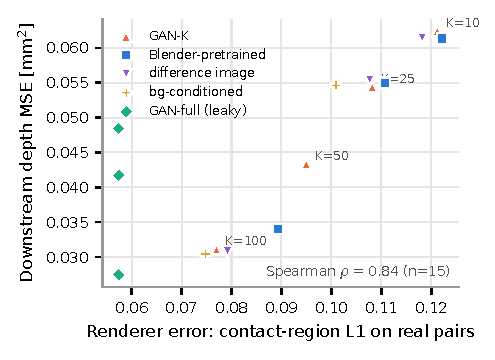
\includegraphics[width=0.9\columnwidth]{figures/fig_fidelity.pdf}
    \caption{\textbf{Renderer fidelity predicts downstream error.} Contact-region L1 between rendered and real images on held-out real (depth, image) pairs versus depth MSE of the downstream model trained with that renderer's synthetic data, for nine renderer variants. The relation is monotone; a renderer can be screened in minutes without downstream training.}
    \label{fig:fidelity}
\end{figure}

\noindent\textbf{A fidelity proxy.} Because every renderer maps depth to image, we can render the depth maps of the real validation pairs and compare with the real images directly. Fig.~\ref{fig:fidelity} plots the contact-region L1 of nine renderer variants against the downstream depth MSE obtained with their synthetic data: the ordering is preserved across families and budgets. The full-image L1 is dominated by the illumination field and is less predictive. This proxy costs seconds per renderer and we used it to screen the variants below before any downstream training.

\begin{table}[t]
\centering
\tableformat
\caption{\textbf{Appearance-side variants} at $\Kreal=25$ (real validation split) and leave-object-out (unseen objects). Renderer fidelity is the contact-region L1 of Fig.~\ref{fig:fidelity}. None of the variants improves contact depth without leakage.}
\label{tab:variants}
\begin{tabularx}{\columnwidth}{Xrrrr}
\toprule
& \multicolumn{2}{c}{$\Kreal=25$} & \multicolumn{2}{c}{Unseen objects} \\
\cmidrule(lr){2-3}\cmidrule(lr){4-5}
Variant & \shortstack[c]{\strut Fidelity\\\strut $\downarrow$} & \metrichead{Contact}{MAE} & \metrichead{Contact}{MAE} & \metrichead{Rot.}{(deg)} \\
\midrule
Real only & -- & 0.303 & 0.347 & 48.3 \\
Real only, bg-norm. & -- & 0.302 & 0.350 & 50.9 \\
GAN-$\Kreal$ / GAN-LOO & 0.108 & 0.318 & 0.333 & 7.6 \\
\quad Blender-pretrained & 0.111 & 0.335 & 0.356 & 8.5 \\
\quad difference-image & 0.108 & 0.339 & 0.346 & 6.3 \\
Blender & -- & 0.347 & 0.352 & 7.8 \\
Blender, bg-norm. & -- & 0.343 & 0.348 & 5.6 \\
\bottomrule
\end{tabularx}
\end{table}

\noindent\textbf{Which appearance factor limits few-shot fidelity?}
\label{sec:negative}
We tested three hypotheses (Table~\ref{tab:variants}).
\emph{(i) Missing physical prior.} A learned renderer with few pairs may lack the depth-to-shading structure that the physical renderer has for free. We pretrained the GAN on $30$k (depth, Blender image) pairs and fine-tuned it on the $\Kreal$ real pairs. Fidelity did not improve at any $\Kreal$ ($0.111$ vs.\ $0.108$ at $\Kreal=25$; $0.089$ vs.\ $0.077$ at $\Kreal=100$) and downstream depth was unchanged or worse.
\emph{(ii) Session illumination drift.} Because each object is one session, we measured the no-contact background of every session (per-pixel median over its frames). The backgrounds differ strongly: the mean blue channel ranges from $0.11$ to $0.38$ across sessions, and the between-session background difference ($0.05$--$0.10$ L1) exceeds the total error of the best renderer ($0.03$). A depth-conditioned renderer cannot know the session, so we normalized every frame (real and simulated) to a canonical background, $I \leftarrow I - B_{\mathrm{session}} + \bar B$, and trained a difference-image GAN that predicts $I-B_{\mathrm{session}}$. Full-image L1 improved by $13$--$21\%$, confirming the drift is real, but contact-region L1 did not move ($0.108$ at $\Kreal=25$) and contact MAE did not improve. The frozen sensor-invariant encoder is already robust to the illumination field; the only downstream effect of normalization is on pose transfer to unseen objects ($7.8^\circ\!\to\!5.6^\circ$ with the physical renderer), where a consistent background removes a spurious cue.
\emph{(iii) Contact shading.} What remains is the appearance \emph{inside} the contact region: the dark, low-contrast, gel-specific shading visible in the real column of Fig.~\ref{fig:renders}, which the physical renderer models with a hand-tuned darkening term and the learned renderer must learn from examples. Every result above is consistent with this being the limiting factor: strict renderers separate from real-only training only when they have seen enough contacts ($\Kreal\!\ge\!100$), leakage helps exactly because it exposes the test contacts, and the downstream errors are localization errors of the contact region (IoU $0.6$--$0.75$) rather than depth-magnitude errors (peak error $<0.1\,$mm).

\section{Discussion and Conclusion}

\noindent\textbf{What simulation buys, and for which task.}
\emph{Pose} needs coverage of the object's contact silhouettes over the pose space, which the geometry stage provides regardless of appearance: a physical renderer fitted to one no-contact frame makes the pose of a new object estimable, covering the rotation range matters more than rendering quality, and simulation keeps pose stable across sessions. \emph{Depth and normals} depend on the appearance inside the contact, which only a learned renderer reproduces, and only after $\approx\!25$--$50$ labeled contacts per object; below that nothing leakage-free helps, above $\approx\!100$ real data alone is already good. Choose by task: for pose of known meshes, calibrate a physical renderer from a background frame and cover the rotations; for dense geometry, budget the real pairs the learned renderer needs, condition it on the session background so that new sessions and objects cost one frame, and account for those pairs when reporting.

\noindent\textbf{Reporting.}
Learned-renderer results should state the renderer's real training set and keep it disjoint from the downstream test frames. On our data the leaky protocol overstates the depth benefit by $2$--$4\times$ where the pipeline is most attractive, and manufactures a $30\%$ gain on unseen objects that no leakage-free renderer reproduces. The contact-region fidelity proxy makes the strict protocol cheap: nineteen renderer variants were ranked without downstream training, and the ranking held.

\noindent\textbf{Limitations.}
Sensor-A data have one session per object, so object identity and session appearance are confounded in the leave-object-out study; the second session and sensor separate them only partially (re-estimated poses, a different capture protocol). Depth references are mesh projections, not membrane measurements. The downstream model is one frozen-encoder architecture; a trainable encoder may extract more from synthetic data or be more sensitive to its artifacts. The physical renderer uses a geometric gel model; a mechanical model could improve the contact shading we identify as the bottleneck.

\noindent\textbf{Conclusion.}
We compared a physically calibrated and a learned tactile renderer on two fingertip sensors, three tasks and four transfer protocols, under a rule that charges each renderer for the real data it consumes and forbids it from seeing the test frames. Simulation transfers tactile pose estimation to objects without real data and stabilizes it across sessions with a renderer calibrated from a single frame; dense depth and normals improve only with a learned renderer and a moderate real budget, on both sensors, and the benefit is overstated by up to $4\times$ when the renderer sees the test distribution. A background-conditioned learned renderer and rotation coverage extend the useful range at no extra labeled data, while physics-guided, illumination-normalized and difference-image renderers do not; the few-shot gap lies in the shading inside the contact.


\bibliographystyle{IEEEtran}
\bibliography{refs}

\end{document}
